\title{CFD laboratory 2\\Turbulent flow development between two parallel plates}
\author{
        Sergio M. Vanegas A.\\
        Francesco de Pas\\
                Department of Mathematics\\
        Polimi---Politecnico di Milano\\
        Milano, Italia
}
\date{\today}

\documentclass[12pt]{article}

\usepackage{amsmath}
\usepackage{graphicx}
\usepackage{siunitx}

\begin{document}
\maketitle

\begin{abstract}
        The present case concerns the development of the turbulent flow between two parallel plates. The flow develops from a condition of uniform velocity (rectangular profile) imposed at the inlet boundary, reaching a fully-developed state at a certain distance from the inlet, and it does not change further downstream until the outlet section. Unlike that in the laminar regime (plane Poiseuille flow), the turbulent flow between two parallel plates does not have any analytical solution. In this laboratory, PHOENICS is used to simulate the flow by solving the RANS coupled with the \( k \text{-} \epsilon\) standard turbulence model and the equilibrium wall function of Launder and Spalding. \cite{FL:03}

        \begin{figure}[ht!]
                \centering
                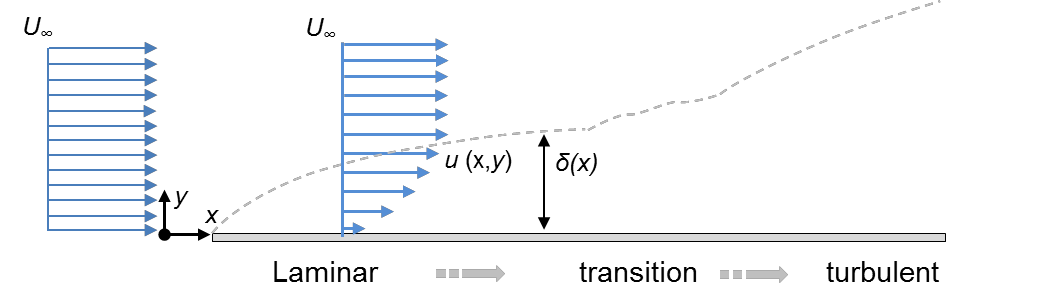
\includegraphics[width=\textwidth]{Sketch.png}
                \caption{Sketch of the test case}
                \label{fig:sketch}
        \end{figure}

\end{abstract}

\section{Introduction}
        \subsection{Flow Domain}

                The symmetry of the Reynolds-averaged flow can be exploited by solving over half of the system and imposing a symmetry condition on the half mid-plane (Figure~\ref{fig:domain}). As for the earlier test case, the inlet should not be placed in direct contact with the plate to avoid numerical issues at the bottom-left corner.

                \begin{figure}[ht!]
                        \centering
                        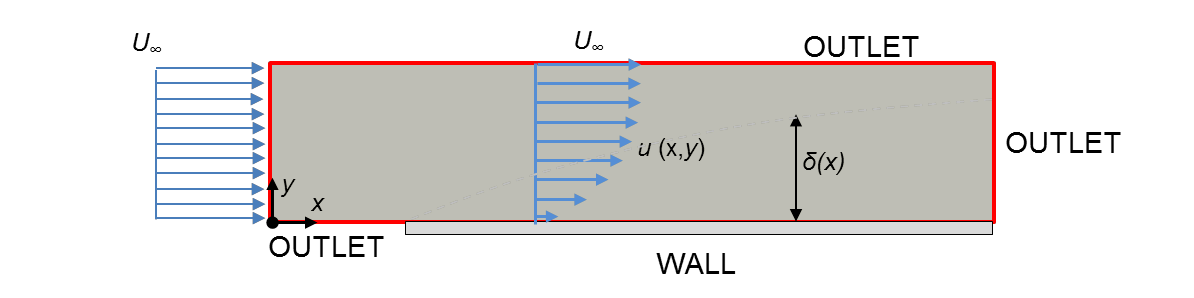
\includegraphics[width=\textwidth]{Domain.png}
                        \caption{Computational domain and boundary conditions}
                        \label{fig:domain}
                \end{figure}

                When defining the CFD model particular attention must be paid in choosing the proper boundary conditions, which are, in this case, inlet, outlet, solid walls and symmetry.

                \begin{itemize}
                        \item At the inlet, a uniform x-velocity profile equal to \( U_b \) is imposed, whereas the y-velocity and z-velocity components are specified as zero. No turbulence shall be assumed at the inlet boundary; this is achieved by setting an intensity \( TI \) equal to 0.
                        \item At the outlet, a zero external \( P^* \) is imposed. Note that the value of \( P^* \) at the outlet will not be zero owing to the presence of a finite outlet coefficient. In order to have \(P_{\text{outlet}}^* = P_{\text{ext}}^* = 0\), set the outlet coefficient to a very large value (e.g. \num{1e+10}). This is not really necessary, however.
                        \item At the solid walls, owing to the no-slip condition, the fluid velocity is zero. In the Finite Volume Framework with staggered-grid arrangement, only the y-velocity at the wall is imposed. The no-slip condition is imposed for the x-velocity indirectly. On the one hand, the advection flux of variable \( U \) through the near-wall cell faces is set to zero. On the other hand, the diffusion flux of variable \( U \) through the near-wall cell faces (that is, the wall shear force) is specified by obtaining the wall shear stress from the equilibrium wall function of Launder and Spalding. Note that the equilibrium wall function requires the dimensionless wall distance of the first grid nodes to be greater than 30 (and generally lower than about 130). Note that the dimensionless wall distance can be calculated only a posteriori.
                \end{itemize}
        
        \subsection{Data of the Problem}

                \begin{itemize}
                        \item Distance between the plates is \( h = \SI{1e-1}{\metre} \)
                        \item Bulk-mean velocity is \( U_b = \SI{1e0}{\metre \per \second} \)
                        \item Working fluid is water at \( \SI{2e1}{\celsius} \), treated as incompressible (\( \rho = \SI{9.9823e2}{\kilogram \per \metre \cubed} , \nu = \SI{1e-6}{\metre \squared \per \second} \))
                \end{itemize}
        
        \subsection{Report Structure}

                The remainder of the report is organized as follows: Section~\ref{sec:convergence} addresses the issue of Whole-Field residual convergence, Flow Full-Development and Grid Independence; Section~\ref{sec:qualitative} presents the relevant profiles and simulated scalars for the qualitative assesment of the model physical consistency; finally, Section~\ref{sec:literature} compares the results of the simulation with the theoretical model studied during the lessons.

\section{Convergence of the CFD Solution} \label{sec:convergence}

        All simulations were ran setting up a minimum of 1000 iterations and a maximum of 10000, with a whole-field residual convergence criterion of 0.0001\%. The probe was set in the middle of the channel with respect to the start of the lower boundary plate. Additionally, regarding the grid-independence study, the near-wall cell width was reduced as much as possible while maintaining a \( y^+ \) value higher than 30, which turned out to be \( \SI{2e-3}{\metre} = \frac{\delta}{25} \).

        Then, we had to modify the channel length until it achieved a fully-developed flow; this was evaluated by observing the x-derivative of the horizontal velocity and the vertical velocity profile, and then extending the channel until both of them became persistantly (near) 0. The results of this process can be seen in Figure~\ref{fig:DUDX_Profile} and Figure~\ref{fig:V_Profile}, by which we can determine that $ L = 150 \delta =  \SI{7.5E0}{\metre}$ is a sufficient channel length for our case of study.

        \begin{figure}[ht!]
                \centering
                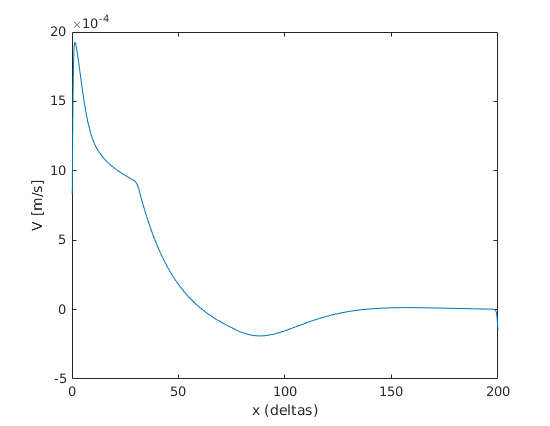
\includegraphics[width=\textwidth]{DUDX_Profile.png}
                \caption{Horizontal velocity X-Derivative Profile}
                \label{fig:DUDX_Profile}
        \end{figure}

        \begin{figure}[ht!]
                \centering
                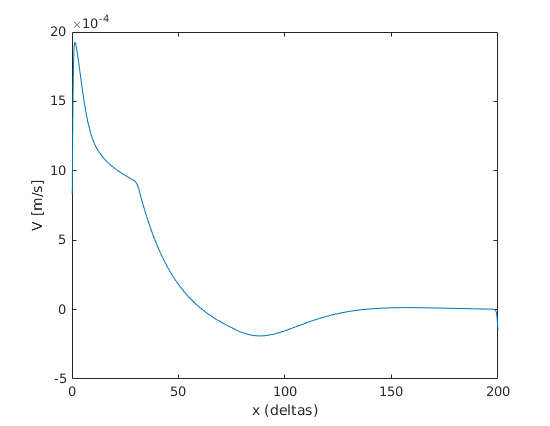
\includegraphics[width=\textwidth]{V_Profile.png}
                \caption{Vertical velocity Profile}
                \label{fig:V_Profile}
        \end{figure}

        Since the \( y^+ \) constraint had already been verified for all of our grid configurations, we then proceeded to study their grid-independence based on the horizontal velocity Y-Profile (inside the fully-developed region) and the Pressure profile across the channel length; these can be seen in Figure~\ref{fig:U_Ind} and Figure~\ref{fig:P_Ind}.respectively. Visually, we can conclude that the variables of interest do converge to a single solution, so that we can state grid-independenceis achieved.

        \begin{figure}[ht!]
                \centering
                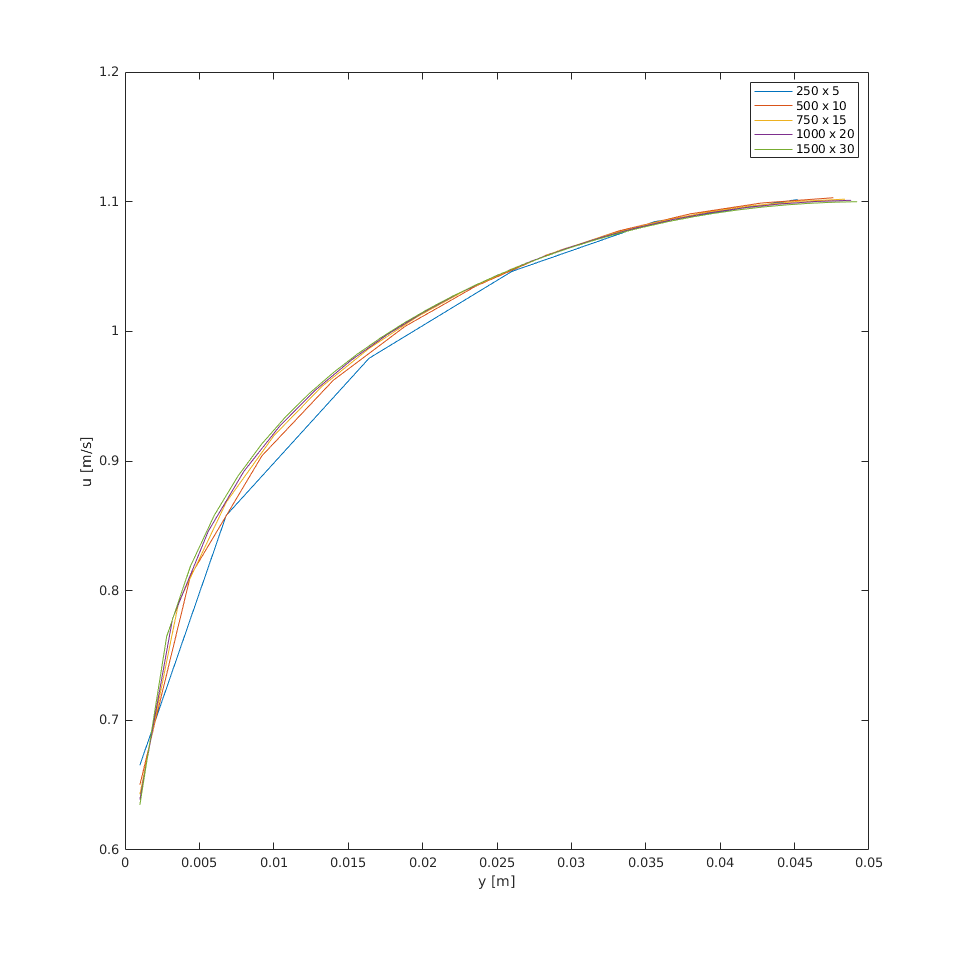
\includegraphics[width=\textwidth]{U_Independence.png}
                \caption{Horizontal velocity Y-Profile}
                \label{fig:U_Ind}
        \end{figure}

        \begin{figure}[ht!]
                \centering
                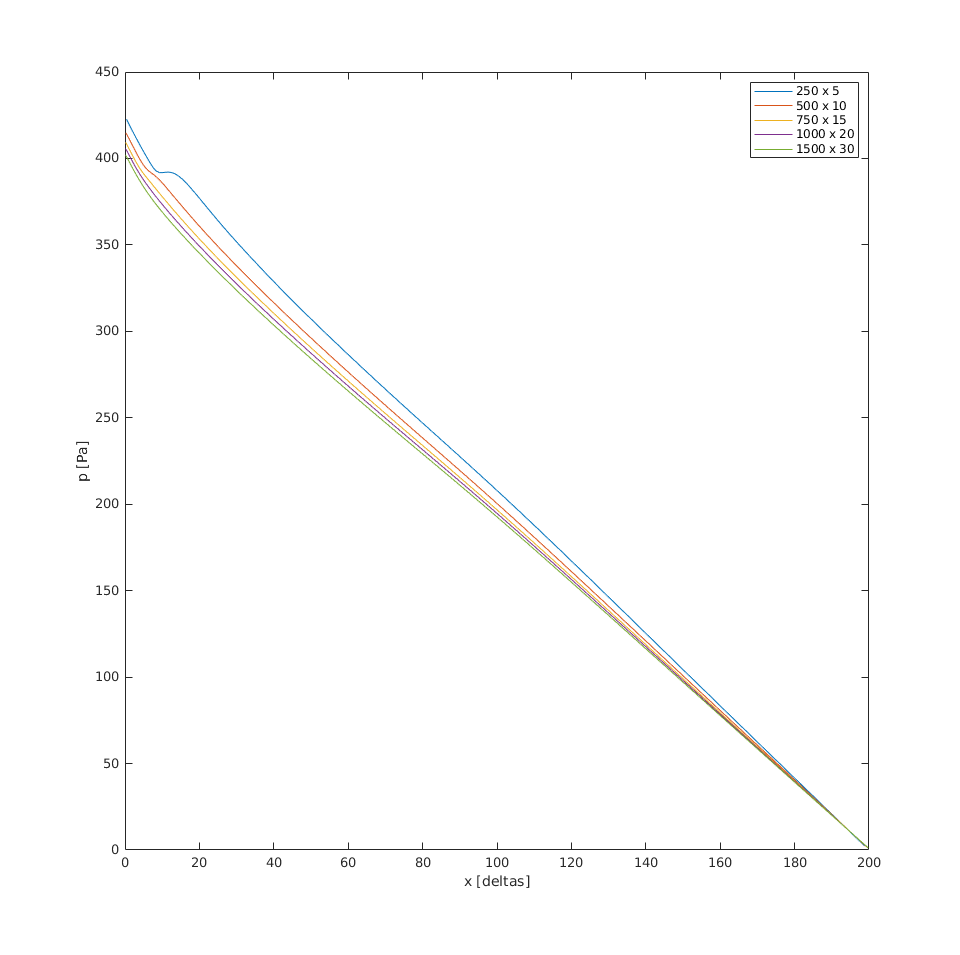
\includegraphics[width=\textwidth]{P_Independence.png}
                \caption{Pressure X-Profile}
                \label{fig:P_Ind}
        \end{figure}

\section{Qualitative assessment of the physical consistency of the CFD solution} \label{sec:qualitative}

        We then proceeded to study the Y-distributions of the stresses; these profiles, as well as the \( \tau_{\text{wall}} \) coefficient, were extracted at \(x \approx 160 \delta\). The viscous shear stress was calculated as in Equation~\ref{eq:visc}, whereas the total shear stress was extracted from the distribution law in Equation~\ref{eq:stress}. The turbulent shear stress was then approximated from the difference between the other two profiles. The resulting plots can be observed in Figure~\ref{fig:stress}

        \begin{equation} \label{eq:visc}
                \tau_{\text{visc}} = \rho \nu \frac{dU}{dy}
        \end{equation}

        \begin{equation} \label{eq:stress}
                \tau = (1 - \frac{y}{\delta}) \tau_{\text{wall}}
        \end{equation}

        \begin{figure}[ht!]
                \centering
                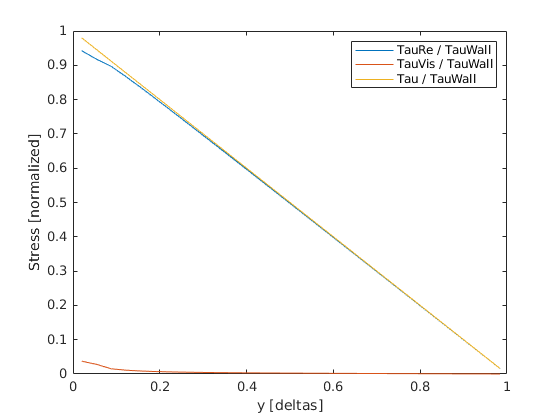
\includegraphics[width=\textwidth]{stress.png}
                \caption{Stress Y-Profiles}
                \label{fig:stress}
        \end{figure}

        Finally, we plotted the normalized Axial (Horizontal) Velocity profile (w.r.t. the centerline velocity) as a function of the normalized channel height against the analytic normalized laminar axial velocity profile w.r.t. the same independent variable; the resulting curves are presented in Figure~\ref{fig:axialV}. As we can observe, the vertical development of the horizontal speed in a turbulent flow is significantly faster close to the wall, and the normalized speed is consistently higher throught the channel section (with the obvious exception of the walls and the channel center).

        \begin{figure}
                \centering
                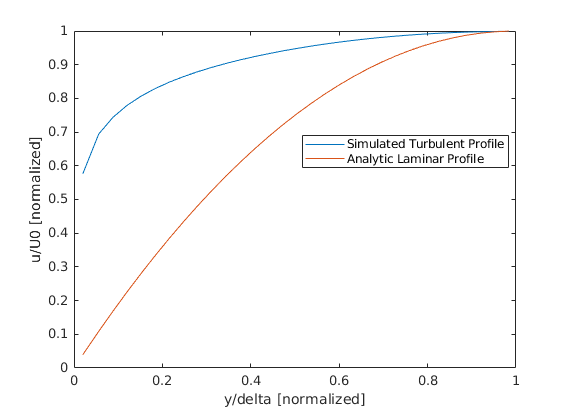
\includegraphics[width=\textwidth]{Axial_Velocities.png}
                \caption{Axial velocity profile comparison}
                \label{fig:axialV}
        \end{figure}

\section{Comparison with literature models} \label{sec:literature}

        Since we kept \( y^+ \) above 30 for all simulations, we were able to use the Log-Law model (described in Equation~\ref{eq:log_law}) to predict the \( u^+ \) profile; the resulting curves plus a vertical line showing the model's limit of operation can be seen in Figure~\ref{fig:u_plus} in a semilogarithmic scale. As one would expect, the simulated curve diverges significantly after this theoretical barrier, but it provides a good first estimate of the profile close to the wall.

        \begin{equation} \label{eq:log_law}
                u^+ = \frac{1}{\kappa} \ln(E y^+) \approx \frac{1}{0.41} \ln(8.6y^+)
        \end{equation}
        
        \begin{figure}
                \centering
                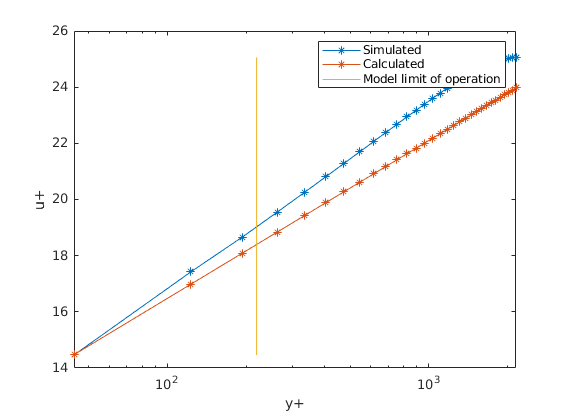
\includegraphics[width=\textwidth]{Up_Profile.png}
                \caption{\( u^+ \) profiles in function of \( y^+ \)}
                \label{fig:u_plus}
        \end{figure}

        We then calculated the skin friction coefficient based on the expression given in Equation~\ref{eq:friction} and plotted both sides of the relation in Equation~\ref{eq:friction_rel} w.r.t. a range of logarithmically spaced values around the previously calculated value, which was in turn drawn as a marker along the aforementioned curves; the result can be observed in Figure~\ref{fig:friction}. Even if not exact, the calculated coefficient from the simulated data provides a fairly accurate estimate of the expected theoretical value.

        \begin{equation} \label{eq:friction}
                c_f = \frac{\tau_w}{\frac{1}{2} \rho U_0^2}
        \end{equation}

        \begin{equation} \label{eq:friction_rel}
                \begin{split}
                        \sqrt{\frac{2}{c_f}} & = \frac{1}{\kappa} \ln \left[ \text{Re} \left( \sqrt{\frac{8}{c_f}} \right)^{-1} \right] + B + B_1 \\
                        & \approx \frac{1}{0.41} \ln \left[ \num{1E5} \left( \sqrt{\frac{8}{c_f}} \right)^{-1} \right] + 5.2 + 0.5
                \end{split}
        \end{equation}

        \begin{figure}
                \centering
                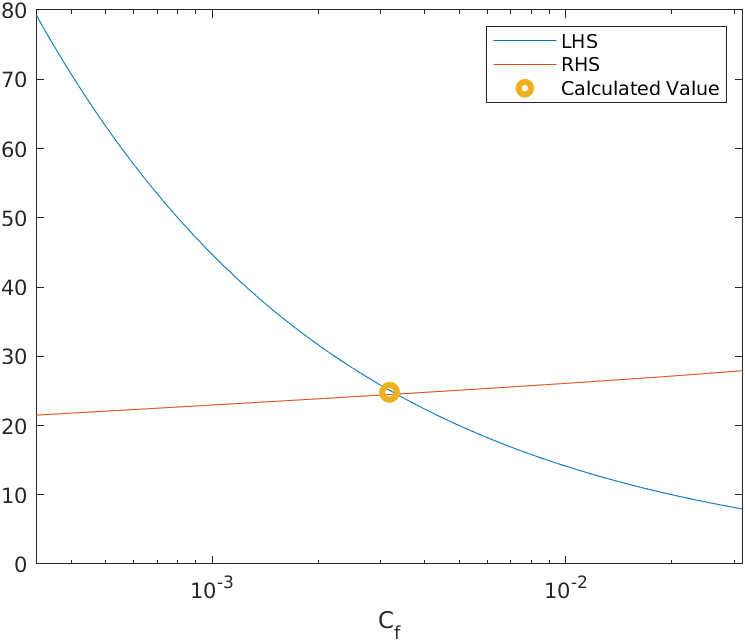
\includegraphics[width=\textwidth]{friction.png}
                \caption{Friction coefficient relations}
                \label{fig:friction}
        \end{figure}

\bibliographystyle{abbrv}
\bibliography{main}

\end{document}
